%%%%%%%%%%%%%%%%%%%%%%% file template.tex %%%%%%%%%%%%%%%%%%%%%%%%%
%
% This is a template file for Web of Conferences Journal
%
% Copy it to a new file with a new name Surname_MESON2016.tex
% and use it as the basis for your article
%
%%%%%%%%%%%%%%%%%%%%%%%%%% EDP Science %%%%%%%%%%%%%%%%%%%%%%%%%%%%
%
%%%\documentclass[option comma separated list]{webofc}
%%%Three important options:
%%% "epj" for EPJ Web of Conferences Journal
%%% "twocolumn" for typesetting an article in two columns format (default one column)
\documentclass[epj]{webofc}

\usepackage[varg]{txfonts}   % Web of Conferences font
%
% Put here some packages required or/and some personnal commands
%
\usepackage{fancyhdr}
\usepackage{subfig}
\usepackage{floatrow}
\usepackage{float}
\usepackage{amsmath}
\usepackage{amssymb}
\usepackage{slashed}
\usepackage{graphicx}
\usepackage{todonotes}
\usepackage[toc,page]{appendix}
\usepackage{hyperref}
\usepackage{placeins}
\usepackage{cleveref}
\usepackage{multirow}
\usepackage{caption}

\def\etaP{\eta^{\prime}}
\def\epem{e^+e^-}

\woctitle{MESON2016 - the 14$^\textrm{th}$ International Workshop on Meson Production, Properties and Interaction}
%
%
\begin{document}
%
\selectlanguage{english}
\title{Light Meson Decays from Photon-Induced Reactions with CLAS}

% insert email only for speaker/presenter
\author{Michael C. Kunkel\inst{1}\fnsep\thanks{\email{m.kunkel@fz-juelich.de}}         
% comment out the next line if not needed
       \\for the CLAS Collaboration
}

\institute{Forschungszentrum J\"ulich, J\"ulich Germany
          }

\abstract{%Do not break line here!
Photoproduction experiments with the CEBAF Large Acceptance Spectrometer CLAS at the Thomas Jefferson National Facility produce data sets with competitive statistics of light mesons. With these data sets, measurements of transition form factors for $\eta$, $\omega$, and $\eta^\prime$ mesons via conversion decays can be performed using the invariant mass distribution of the final state dileptons. Tests of fundamental symmetries and information on the light quark mass difference can be performed using a Dalitz plot analysis of the meson decay. An overview of preliminary results, from existing CLAS data, and future prospects within the newly upgraded CLAS12 apparatus are given.
}
%
\maketitle
%
\section{Introduction}
\label{intro}
Decays of light mesons provide insight into the structure of the meson. The Light Meson Decay (LMD) group, established at the Thomas Jefferson National Facility with worldwide collaboration, investigates physics pertaining to, but not limited to, transition form factors, anomalous decays and the search for CP violation through Dalitz plot analysis. The presentation given was an overview of the LMD program, recent updates on measurements and an outlook on measurements that can be taken with the \textsc{\texttt{CLAS12}} detector. 
\section{Light Meson Decay Program}
The light meson group was established in 2013. The goal of the group is to investigate properties of light meson decays using data obtained with the \textsc{\texttt{CLAS}} detector.
%Figure~\ref{fig:clas} shows the \textsc{\texttt{CLAS}} detector and its components.
%\begin{figure}[ht]
%\centering
%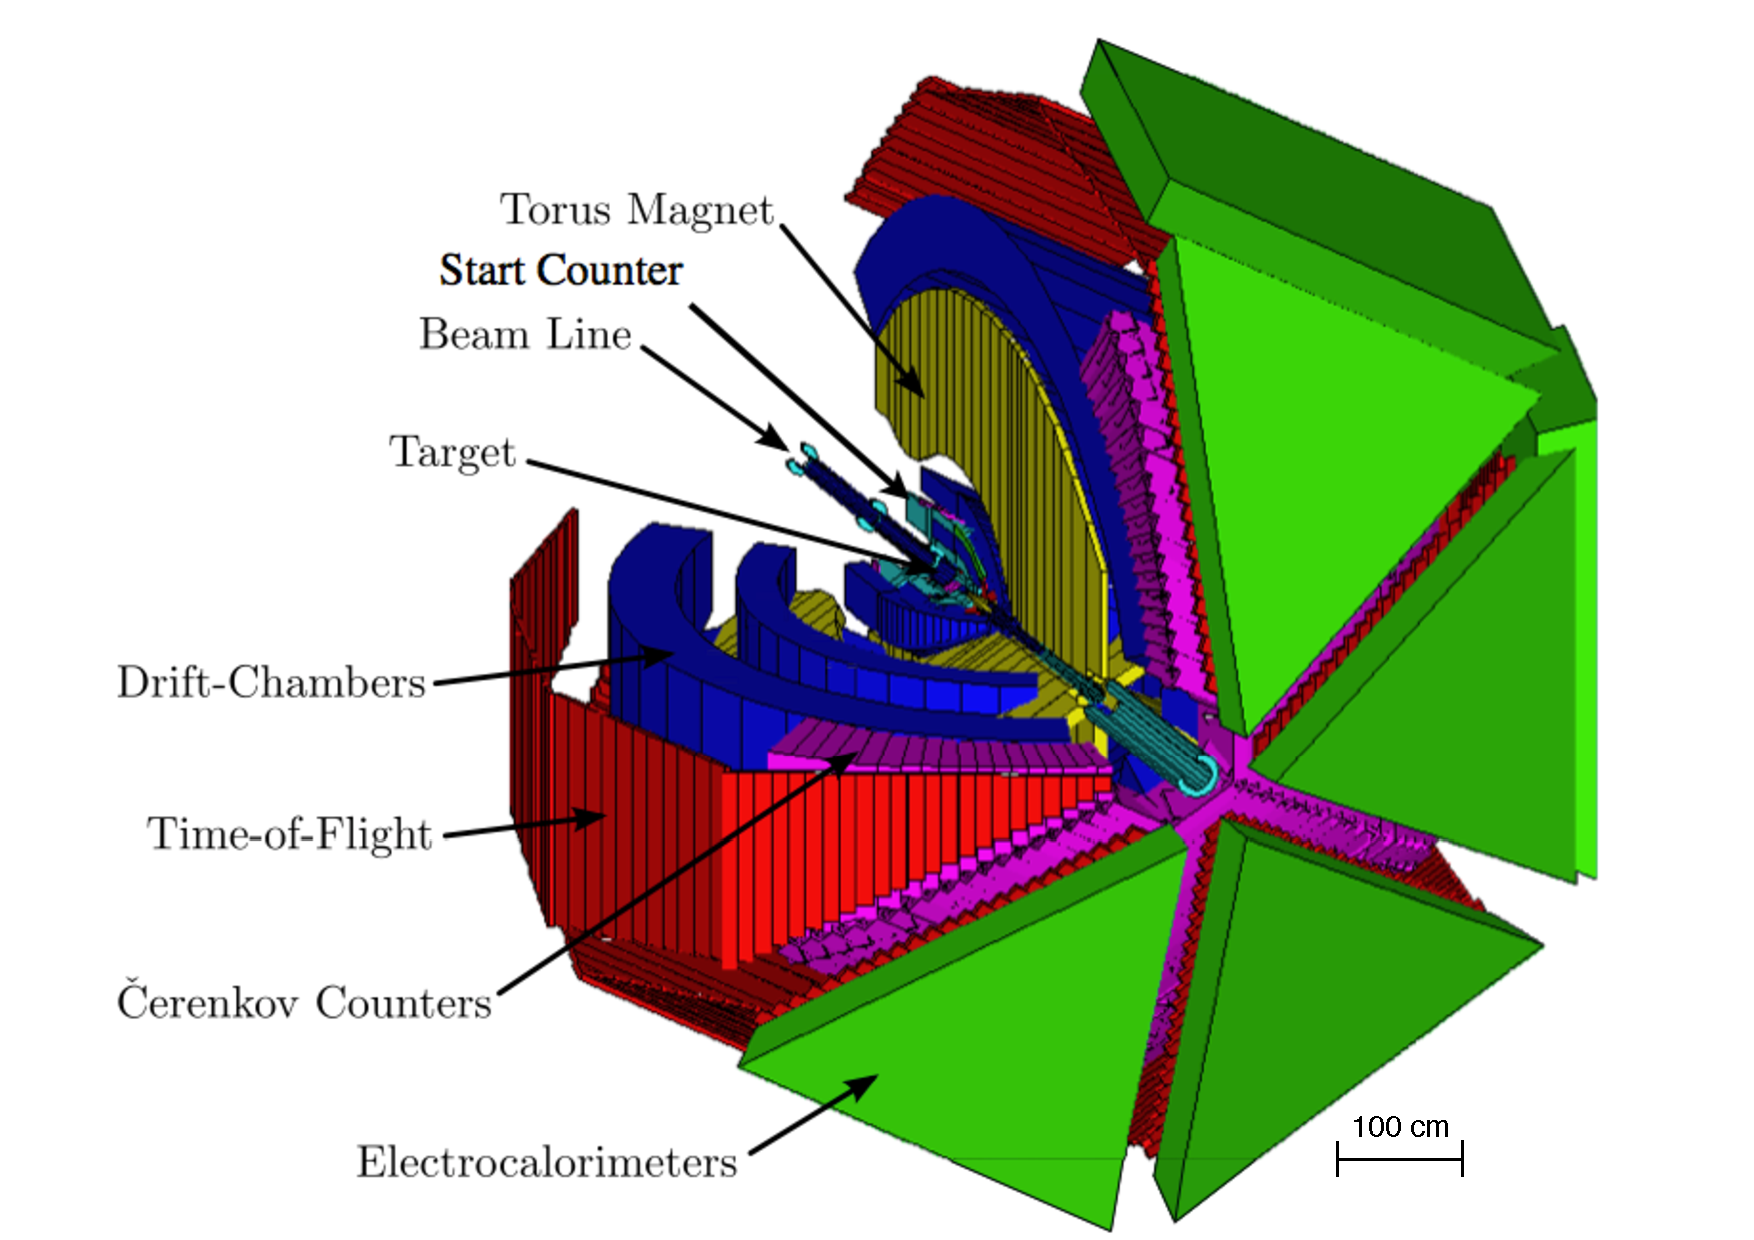
\includegraphics[width=175 pt,clip]{figures/clas_schematicIII.pdf}
%\caption{The CEBAF Large Acceptance Spectrometer (\textsc{\texttt{CLAS}}).}
%\label{fig:clas}       % Give a unique label
%\end{figure}
Since decays of hadrons are independent of production, all \textsc{\texttt{CLAS}} data can be used, however there are two experiments that were chosen as flagships for the program, the g11 and g12 experiment. Both experiments use a photon beam incident on a liquid hydrogen target which created photo-induced reactions with photon beam energies of 800~MeV - 3.8~GeV for g11 and 1.1~GeV - 5.5~GeV for g12.  See~\cite{lmdCAA} for a complete list of meson decays the LMD group plans to investigate.
%See Table~\ref{tab:lmd.channels} for a list of meson decays the LMD group plans to investigate.
%\begin{table}[h!]
\begin{minipage}{\textwidth}
\begin{center}


\caption{\label{tab:lmd.channels}LMD planned measurements \vspace{0.75mm}}
\begin{tabular}{cc||cc}
%\begin{tabular}{p{5cm} | p{7cm}}
\hline
Meson Decay & Physics Interest &Meson Decay & Physics Interest \\
\hline
$\pi^0\to e^+e^-\gamma$  & Heavy photon upper limit &$\eta^{\prime}\to \pi^+\pi^-\gamma$  & Box anomaly \\
$\eta^{\prime}\to e^+e^-\gamma$  & Transition form factor &$\omega\to \pi^+\pi^-\gamma$  & Upper limit branching ratio \\
$\omega\to e^+e^-\pi^0$ & Transition form factor & $\eta, \omega, \phi\to \pi^+\pi^-\pi^0$ & Dalitz plot analysis\\
$\eta^{\prime}\to e^+e^-\pi^0$ & C violation & $\eta^{\prime}\to \pi^+\pi^-\eta$ & Dalitz plot analysis\\
$\eta^{\prime}\to e^+e^-\pi^+\pi^-$  & CP violation & $\phi\to \pi^+\pi^-\eta$ & G-parity violation\\
\hline 
\end{tabular}


\end{center}
\end{minipage}
\end{table}
\vspace{20pt}
\subsection{The Radiative Decay of the $\eta$ and $\eta^\prime$  Meson}
The two-photon decay of the pseudoscalar mesons $\pi^0, \eta , \eta^{\prime} \to \gamma \gamma $ proceed via the triangle or axial anomaly. Radiative decays of  $\eta , \ \eta^{\prime} \to \pi^+ \pi^- \gamma $ are related to the box anomaly. The radiative decay widths of $ \eta^{\prime}$ and $\eta^{\prime}$ are determined by the box anomaly in the chiral limit by 
Eq.~\ref{eq:decaywidth};
\begin{equation}
\frac{d\Gamma (\eta^{(\prime)} \to \pi^+ \pi^- \gamma)}{ds_{\pi\pi}} = A\vert P(s_{\pi\pi}) F_V(s_{\pi\pi}) \Gamma_0(s_{\pi\pi})\vert  \label{eq:decaywidth} \\
\end{equation}
where $\Gamma_0(s_{\pi\pi})$ is the P-wave phase-space constant, denoted in Eq.~\ref{eq:decayconstant} with $\kappa$ being a 
numerical constant. $F_V(s_{\pi\pi})$ is the pion form factor that can be approximated by Eq.~\ref{eq:decayformfactor} and  
$P(s_{\pi\pi})$ is expanded around the chiral limit, $s_{\pi\pi} = 0$, as in Equation~\ref{eq:decaychiral}, where $\alpha$ is the 
variable of measurement.
\begin{eqnarray}
\Gamma_0(s_{\pi\pi}) = \frac{\kappa \left(M^2_{\eta^{(\prime)}} - s_{\pi\pi} \right)^3  s_{\pi\pi} \left(1- \frac{ 4M^2_{\pi }}{    s_{\pi\pi}  }\right)^{\frac{3}{2}}   }{M^3_{\eta^{(\prime)} }}  \label{eq:decayconstant}  \\
\vert F_V(s_{\pi\pi}) \vert \approx 1+(2.12\pm0.01)s_{\pi\pi} + (2.13\pm0.01)s_{\pi\pi}^2+(13.89\pm0.14)s_{\pi\pi}^3 \label{eq:decayformfactor} \\ \nonumber
\\ 
P(s_{\pi\pi}) = 1 + \alpha s_{\pi\pi} + \mathcal{O}(s_{\pi\pi}^2) \label{eq:decaychiral}
\end{eqnarray}
Previous results on the radiative decay for the $\eta$ meson from WASA-at-COSY~\cite{bib0} and KLOE~\cite{bib1} would profit from further measurements. Only one measurement exists for the $\eta^{\prime}$ radiative decay~\cite{bib2}. With the \textsc{\texttt{CLAS}} g11 experiment, both the $\eta$ and  $\eta^{\prime}$ radiative decay width will be measured. In Figure~\ref{fig:boxCLASdata} the \textsc{\texttt{CLAS}} g11 data is shown for the particle selection of exclusive $\gamma p \to p  \pi^+ \pi^- \gamma $. Selecting events within a $2.5 \sigma$ range of $\eta^{\prime}$ and applying efficiency corrections, the $s_{\pi\pi}$ distribution is shown in Figure~\ref{fig:boxCLAS} along with preliminary fit results using Eq.~\ref{eq:decaychiral} and theory predictions~\cite{Kubis2015}.  
\begin{equation}
s_{\pi\pi} = m^2 - 2E_{\gamma}m \label{eq:spipi} \\
\end{equation}
\begin{figure}[h]
	\centerline{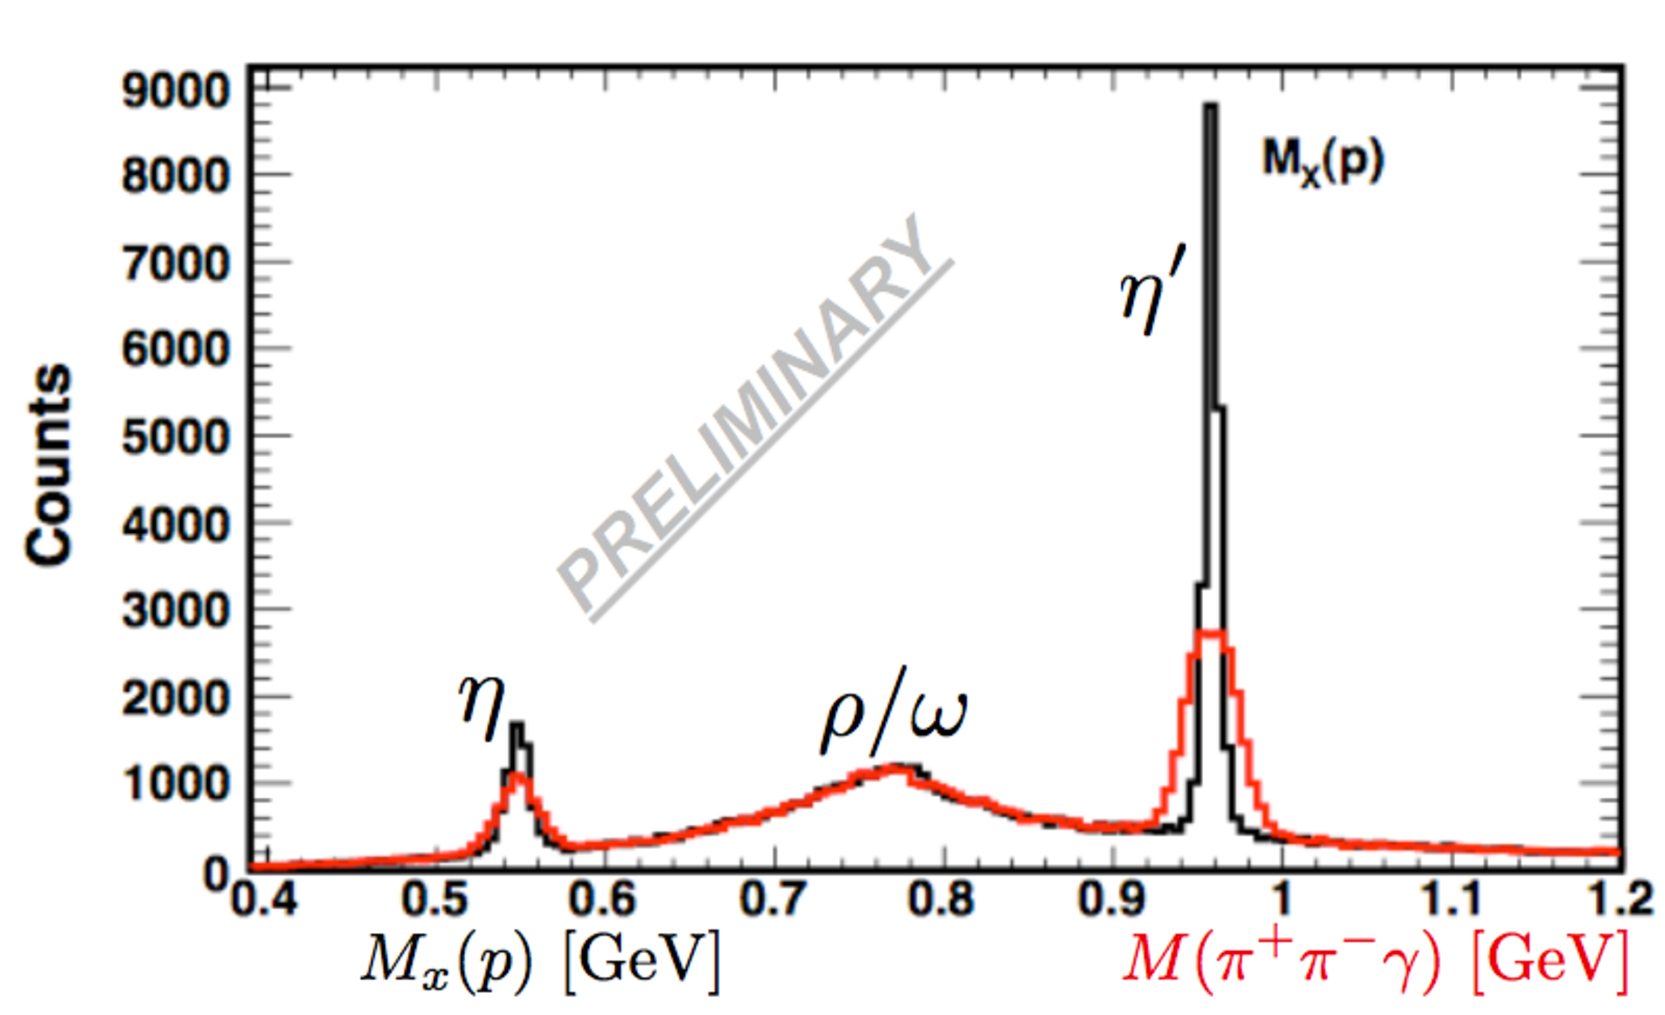
\includegraphics[width=150 pt, height = 100 pt ]{figures/clas_g11data.pdf}}
	\caption{\textsc{\texttt{CLAS}} yield for $\gamma p \to p \eta^{(\prime)} \to p \pi^+ \pi^- \gamma $ from the g11 data set.}
	\label{fig:boxCLASdata}
\end{figure}
\begin{figure}[h!]
	\centerline{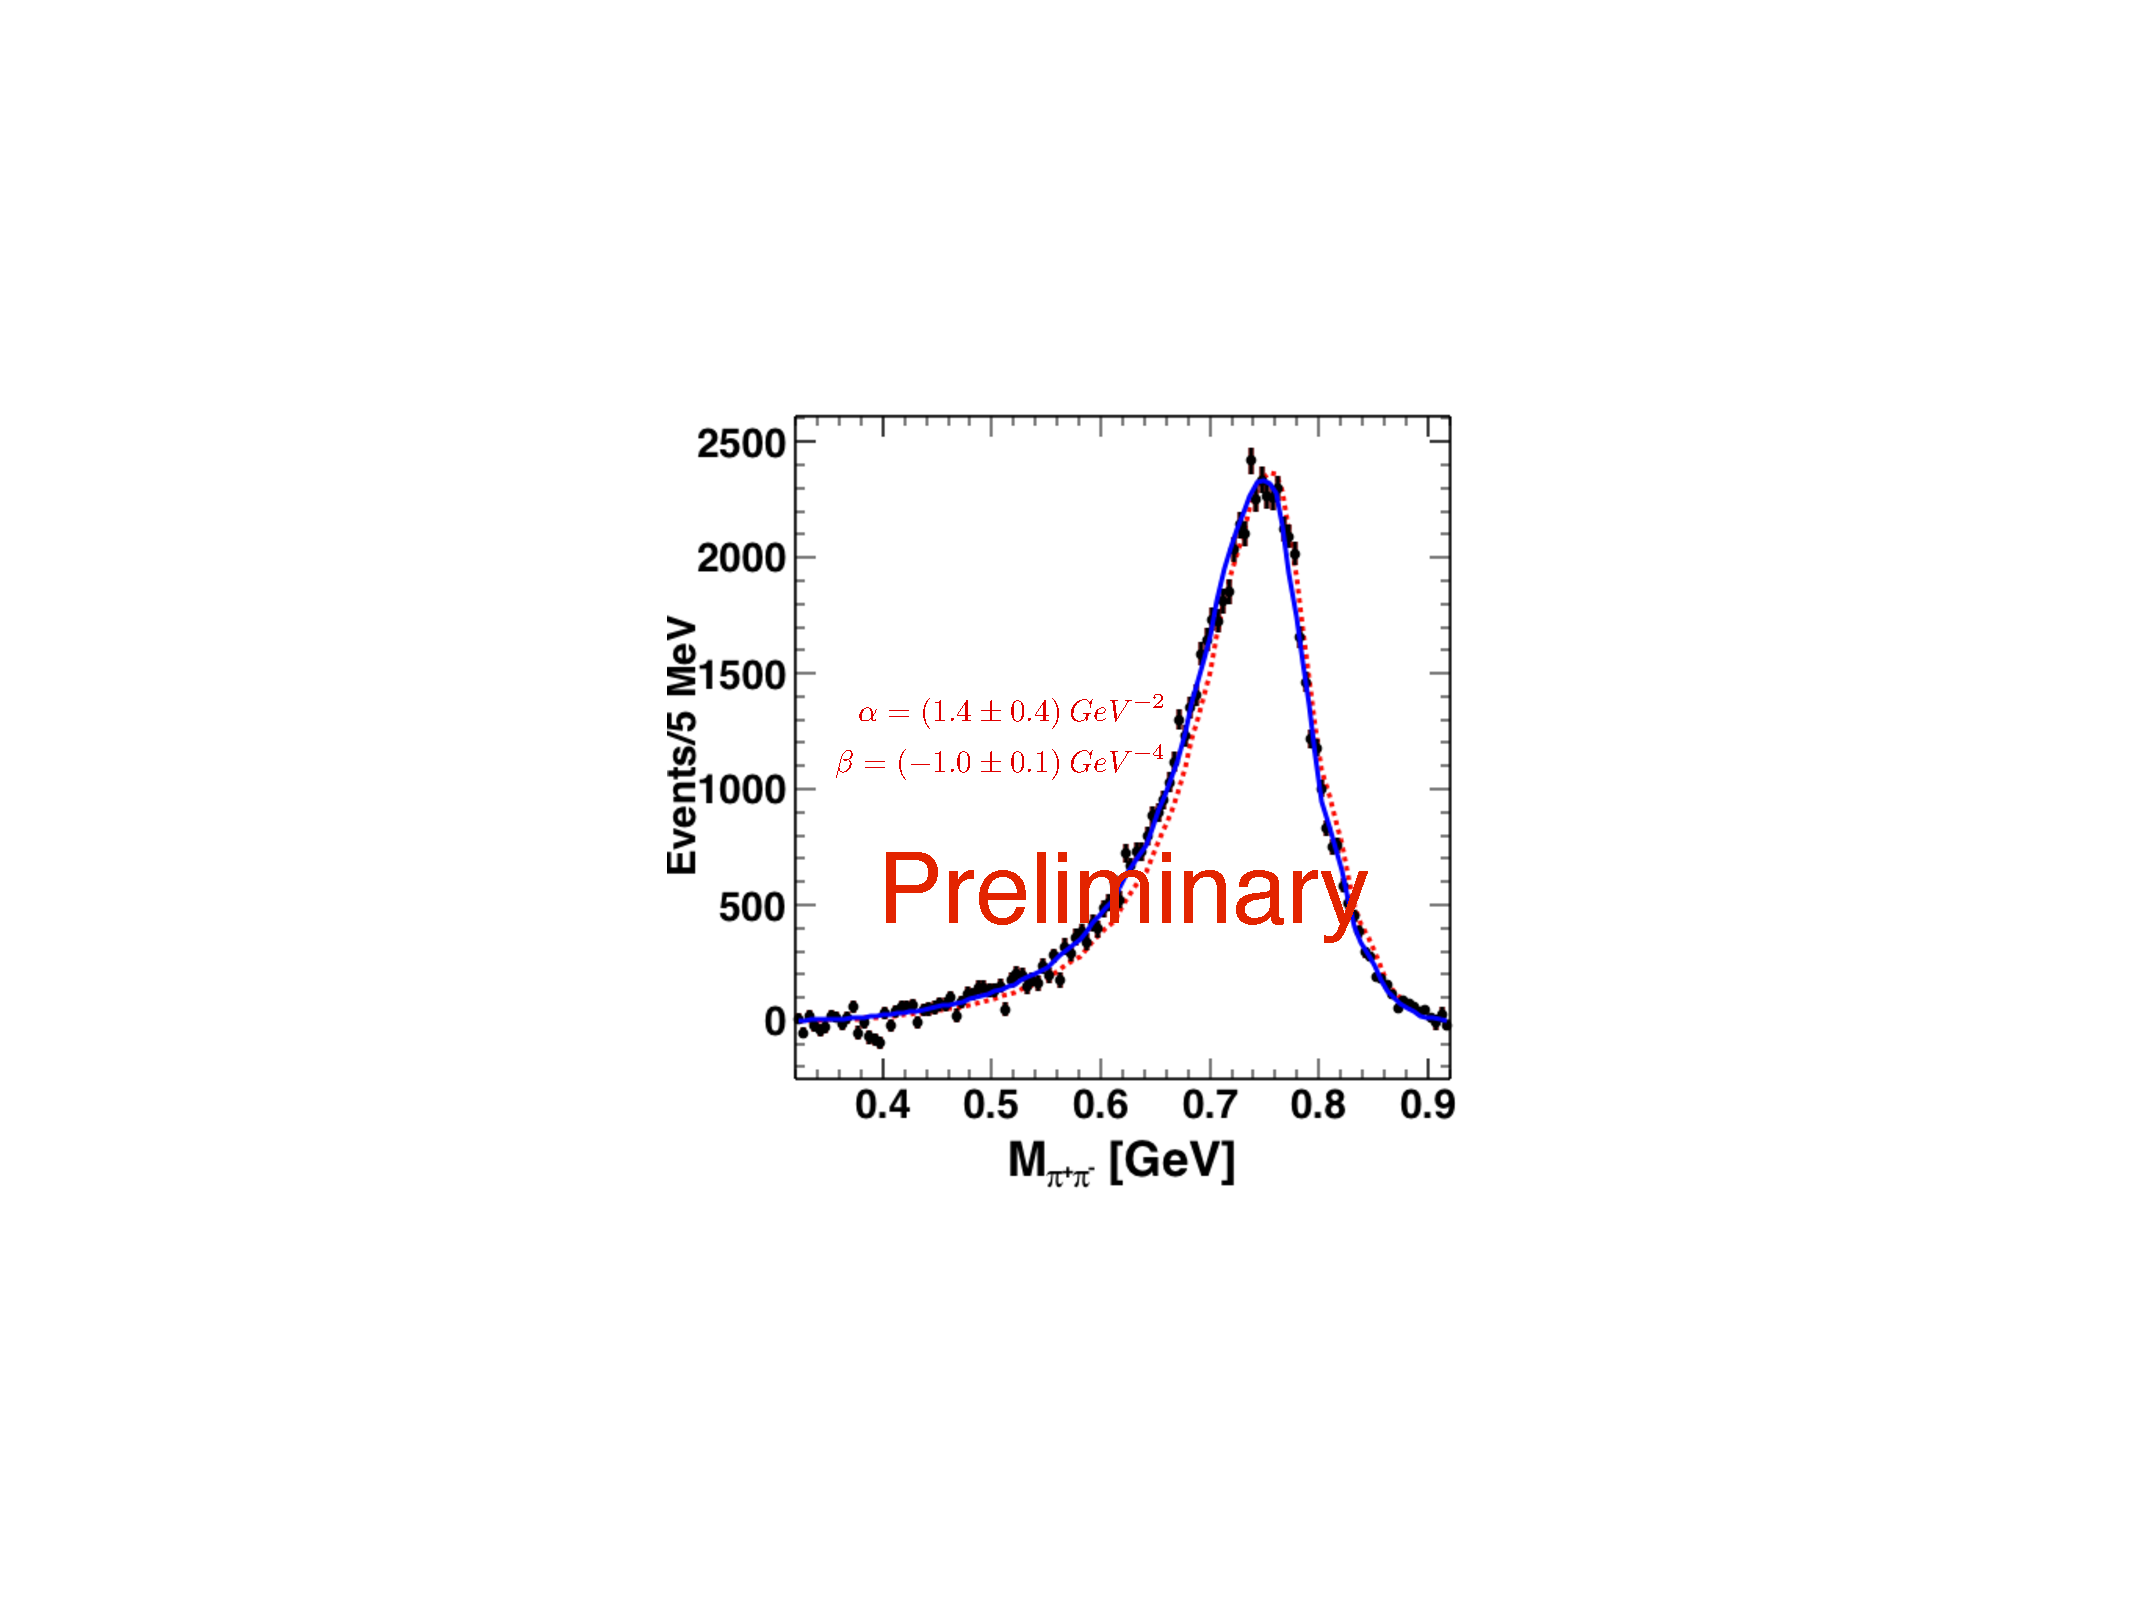
\includegraphics[width=150 pt]{figures/GeorgieLMD_May_06_16_tempIII.pdf}}
	\caption{(black)\textsc{\texttt{CLAS}} preliminary $s_{\pi\pi}$ distribution for $\eta^{\prime}$ with (blue solid line) preliminary fit results using Eq.~\ref{eq:decaychiral} and (red dashed line)theory predictions~\cite{Kubis2015}.}
	\label{fig:boxCLAS}
\end{figure}
\FloatBarrier
\subsection{Update on the Dalitz plot analysis of $\eta^{\prime} \to \pi^+ \pi^- \eta$}
The Dalitz plot of $\eta^{\prime} \to \pi^+ \pi^- \eta$ provides kinematic information of the decay, enabling the study of low energy dynamics of QCD and heavier mass pseudoscalar mesons. The  $\eta^{\prime} \to \pi^+ \pi^- \eta$ decay has a low Q-value due to the decay products being relatively heavy, this helps test and limit the effective chiral Lagrangian theory. The measurable of the Dalitz plot $X$ and $Y$ are projected and fitted to the Equation~\ref{eq:dalitzpro} to extract the parameters $a$, $b$, $c$, $d$. %Table~\ref{tab:dal.parms} shows the previous measurements of Equation~\ref{eq:dalitzpro} along with the projected statistical error a measurement from the CLAS g11 data.
\begin{equation}
f(X,Y) = A(1+a(Y) + b (Y^2) + c(X) + d(X^2)  \label{eq:dalitzpro} \\
\end{equation}
%\begin{table}[h!]
\begin{minipage}{\textwidth}
\begin{center}


\caption{\label{tab:dal.parms}Previous \vspace{0.75mm}}
\begin{tabular}{cccccc}
%\begin{tabular}{p{5cm} | p{7cm}}
\hline
Parameter & VES & Theory & BESIII & Stat. err. in BESIII & Projected CLAS stat. err. \\
\hline
a & -0.127 $\pm$ 0.018 & -0.116 $\pm$ 0.011 & -0.047 $\pm$ 0.012 &$\pm$ 0.011&$\pm$ 0.004 \\
b & -0.106 $\pm$ 0.032 & -0.042 $\pm$ 0.034 & -0.069 $\pm$ 0.021 &$\pm$ 0.019&$\pm$ 0.006\\
c & 0.015                        &                                  & 0.019  $\pm$  0.012 &$\pm$ 0.011&$\pm$ 0.004\\
d & -0.082 $\pm$ 0.019 & -0.010 $\pm$ 0.019 & -0.073 $\pm$ 0.013 &$\pm$ 0.012&$\pm$ 0.004\\
\end{tabular}


\end{center}
\end{minipage}
\end{table}
\vspace{20pt}
This topic was briefly discussed, as a full update was given by later in the session.
\subsection{The Transition Form Factor  of the $\omega$ Meson}
Transition form factors characterize modifications of the point-like photon-meson vertex due to the structure of the meson. The virtual photon can interact with quarks, therefore it can be used as a probe for the internal structure of mesons and its electromagnetic interaction is calculable with the Kroll-Wada formula~\cite{bib4}, Equation~\ref{eq:kroll};
\begin{equation}
\frac{d\Gamma_{M{\rightarrow l^{+}l^{-}X}}}{dq^{2} d\Gamma_{M{\rightarrow X\gamma}}} = \frac{\alpha}{3\pi q^{2}}\left(\left(1+\frac{q^{2}}{m^{2}_{M}-m^{2}_{X}}\right)^2 - \frac{4m^{2}_{M}q^2}{(m^{2}_{M}-m^{2}_{X})^2}\right)^\frac{3}{2}\left(1-\frac{4m_{l}^{2}}{q^{2}}\right)^{1/2}\left(1+\frac{2m_{l}^{2}}{q^{2}}\right) \bigg|_{\mathrm{Q.E.D}}  \label{eq:kroll} \ . \\
\end{equation}
 where $M$ is the species of meson i.e. $\pi^0$, $\eta$, $\omega$, $\eta^{\prime}$, etc., $X$ is the child particle in the decay, $m_M$ the mass of the meson, $m_X$ the mass of the child particle, $m_l$ the mass of the lepton species in the decay, i.e. $e^{\pm}$ or $\mu^{\pm}$ and $q$ being the momentum transfer which is identical to the invariant mass of the dilepton. Deviations of Equation~\ref{eq:kroll} represent the internal structure of the meson for pseudoscalar mesons, while for vector mesons the deviation represents the transition from $M \to X$. These deviations are the transition form factor $\left| F(q^2)\right|$ and can be determined by comparing Equation~\ref{eq:kroll} to what is measured experimentally.
 \begin{equation}
 \frac{d\Gamma_{M{\rightarrow l^{+}l^{-}X}}}{dq^{2} d\Gamma_{M{\rightarrow X\gamma}}}\bigg|_{\mathrm{measured}} =   \frac{d\Gamma_{M{\rightarrow l^{+}l^{-}X}}}{dq^{2} d\Gamma_{M{\rightarrow X\gamma}}} \bigg|_{\mathrm{Q.E.D}} \left| F(q^2)\right|^2 \label{eq:kroll_ff} \ . \\
 \end{equation}
 Depending on the decay width of the meson of interest, the transition can be modeled as a simple pole, Equation~\ref{eq:pole}, a complex pole, Equation~\ref{eq:cpole}, or some other function that describes the transition.
 \begin{eqnarray}
\left| F(q^2)\right| = \frac{1}{1-\frac{q^2}{\Lambda^2}} \label{eq:pole} \\
\left| F(q^2)\right|^2 = \frac{\Lambda^2(\Lambda^2 + \gamma^2)}{(\Lambda^2 - q^2)\Lambda^2 \gamma^2} \label{eq:cpole} \ ,
 \end{eqnarray} 
 where $\Lambda$ and $\gamma$ is the mass and width of the virtual vector meson mass, respectively.
 Recent measurements of the transition form factor for $\omega \to \mu^+\mu^- \pi^0$ have shown unexpected discrepancies with the Vector Dominance Model~\cite{bib5} and recent models of chiral Lagrangian field theory~\cite{bib6}, and dispersion theory~\cite{Schneider} attempt to predict the contributions of the virtual vector meson.
 % as seen in Figure~\ref{fig:omega_ff}.
% \begin{figure}[h!]
% 	\centerline{\includegraphics[width=250 pt, height=130 pt]{figures/omega_ff_bastian_edit.pdf}}
% 	\caption{Form factor of the decay $\omega \to l^+l^- \gamma$ compared to dimuon data by the NA60 Collaboration~\cite{bib5,bib5_0} and LEPS~\cite{LEPS}. Shown are VMD (dotted line) Eqs.~(\ref{eq:kroll},~\ref{eq:cpole}) using the mass of the $\rho$ meson as the virtual vector meson, the results of a chiral Lagrangian treatment with explicit vector mesons~\cite{bib6} (white shaded curve with solid borders), a simplified approximation to the full dispersive solution~\cite{Schneider} (gray shaded curve with dashed borders), full dispersive solution~\cite{Schneider} (black hatched curve with solid borders).~\cite{Schneider}}
% 	\label{fig:omega_ff}
% \end{figure}
 
With the \textsc{\texttt{CLAS}} g12 experiment, lepton ($e^{\pm}$) identification is done using Cherenkov detectors and electromagnetic calorimetry, providing a $e^{+}e^{-}/\pi^{+}\pi^{-}$ rejection of $10^6$. Using the $e^{\pm}$ data from \textsc{\texttt{CLAS}} g12, the $ \omega \to p e^+ e^- \pi^0$ transition form factor can be extracted. Preliminary studies have shown that the number of $ \omega \to p e^+ e^- \pi^0$ events in CLAS to be $\approx 3\cdot 10^3$.
% Figure~\ref{fig:clas_omega_ff} shows the region of the $\omega$ meson.
%\begin{figure}[h!]
%		\centering
%		\centerline{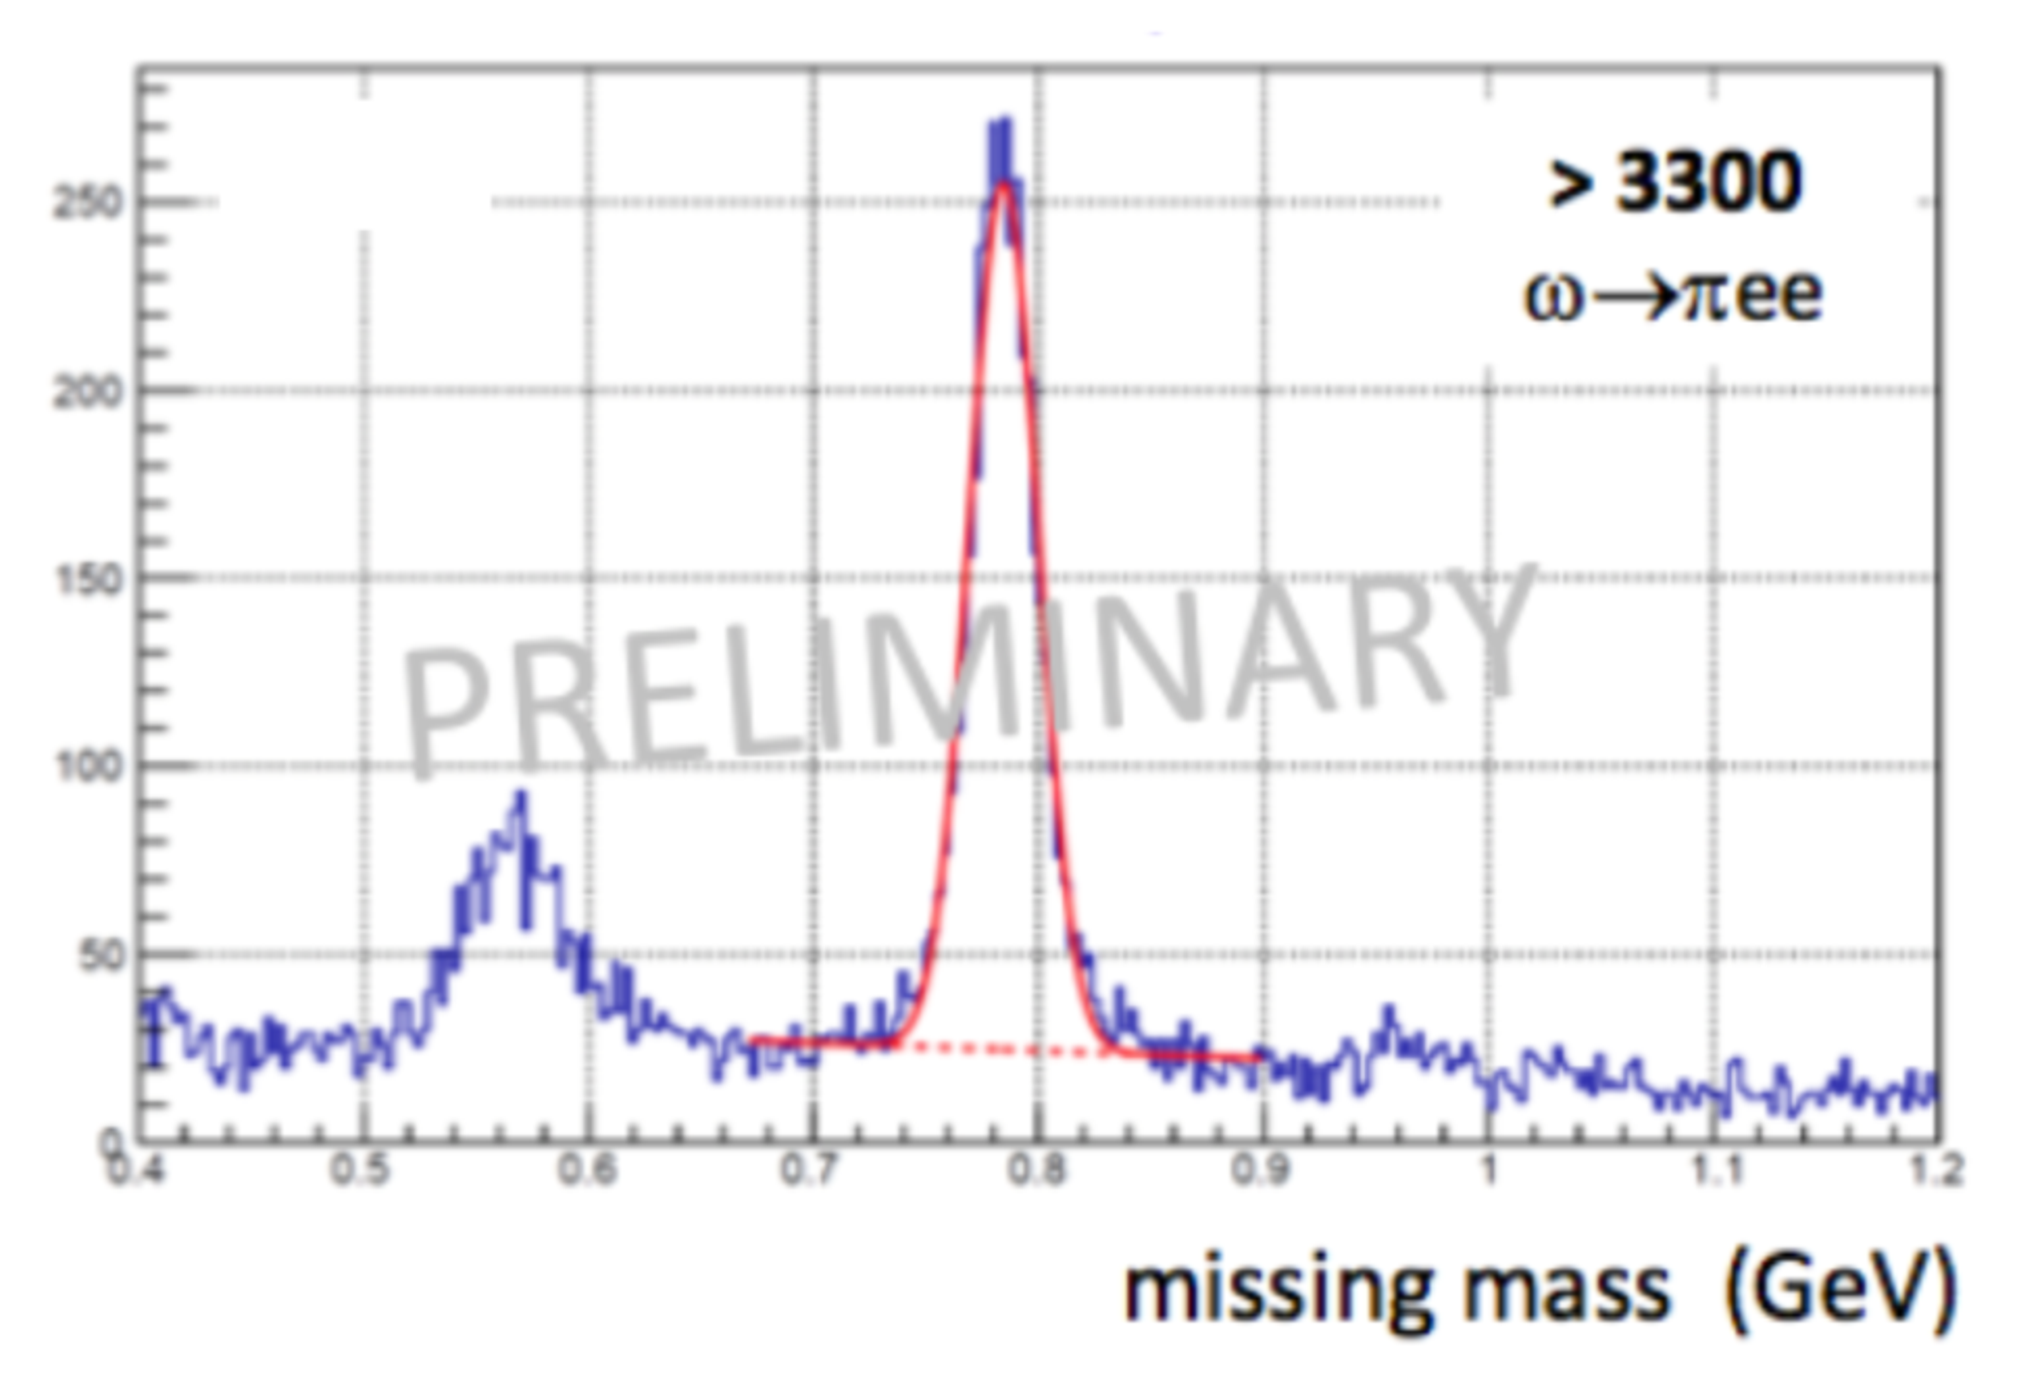
\includegraphics[width=150 pt]{figures/clas_omega_ff_II.pdf}}
%		\caption{\textsc{\texttt{CLAS}} yield for $\gamma p \to p X \to p e^+ e^- \pi^0 $ from g12 data set}{}
%		\label{fig:clas_omega_ff}
%\end{figure}
\FloatBarrier
\subsection{Update on the Branching Ratio Measurement  of the $\eta^\prime \rightarrow e^+e^-\gamma$ Decay}
A recent measurement of BESIII reports the branching ratio $\Gamma(\eta^{\prime} \to  e^+ e^-  \gamma)$/$\Gamma(\eta^{\prime} \to  \gamma  \gamma)$ to be $2.13\pm0.09(stat.)\pm0.07(sys.))10^{-2}$ from 864 events~\cite{bib7}.  Using the $e^{\pm}$ data from \textsc{\texttt{CLAS}} g12, preliminarily 172 events of the $\eta^{\prime} \to  e^+ e^-  \gamma$ decay were observed and analyzed, using the Q-factor~\cite{bib8} method to suppress background from neighboring $A \to e^+ e^-  X$ decays, Figure~\ref{fig:etaP_ff}.
\begin{figure}[h!]
\centerline{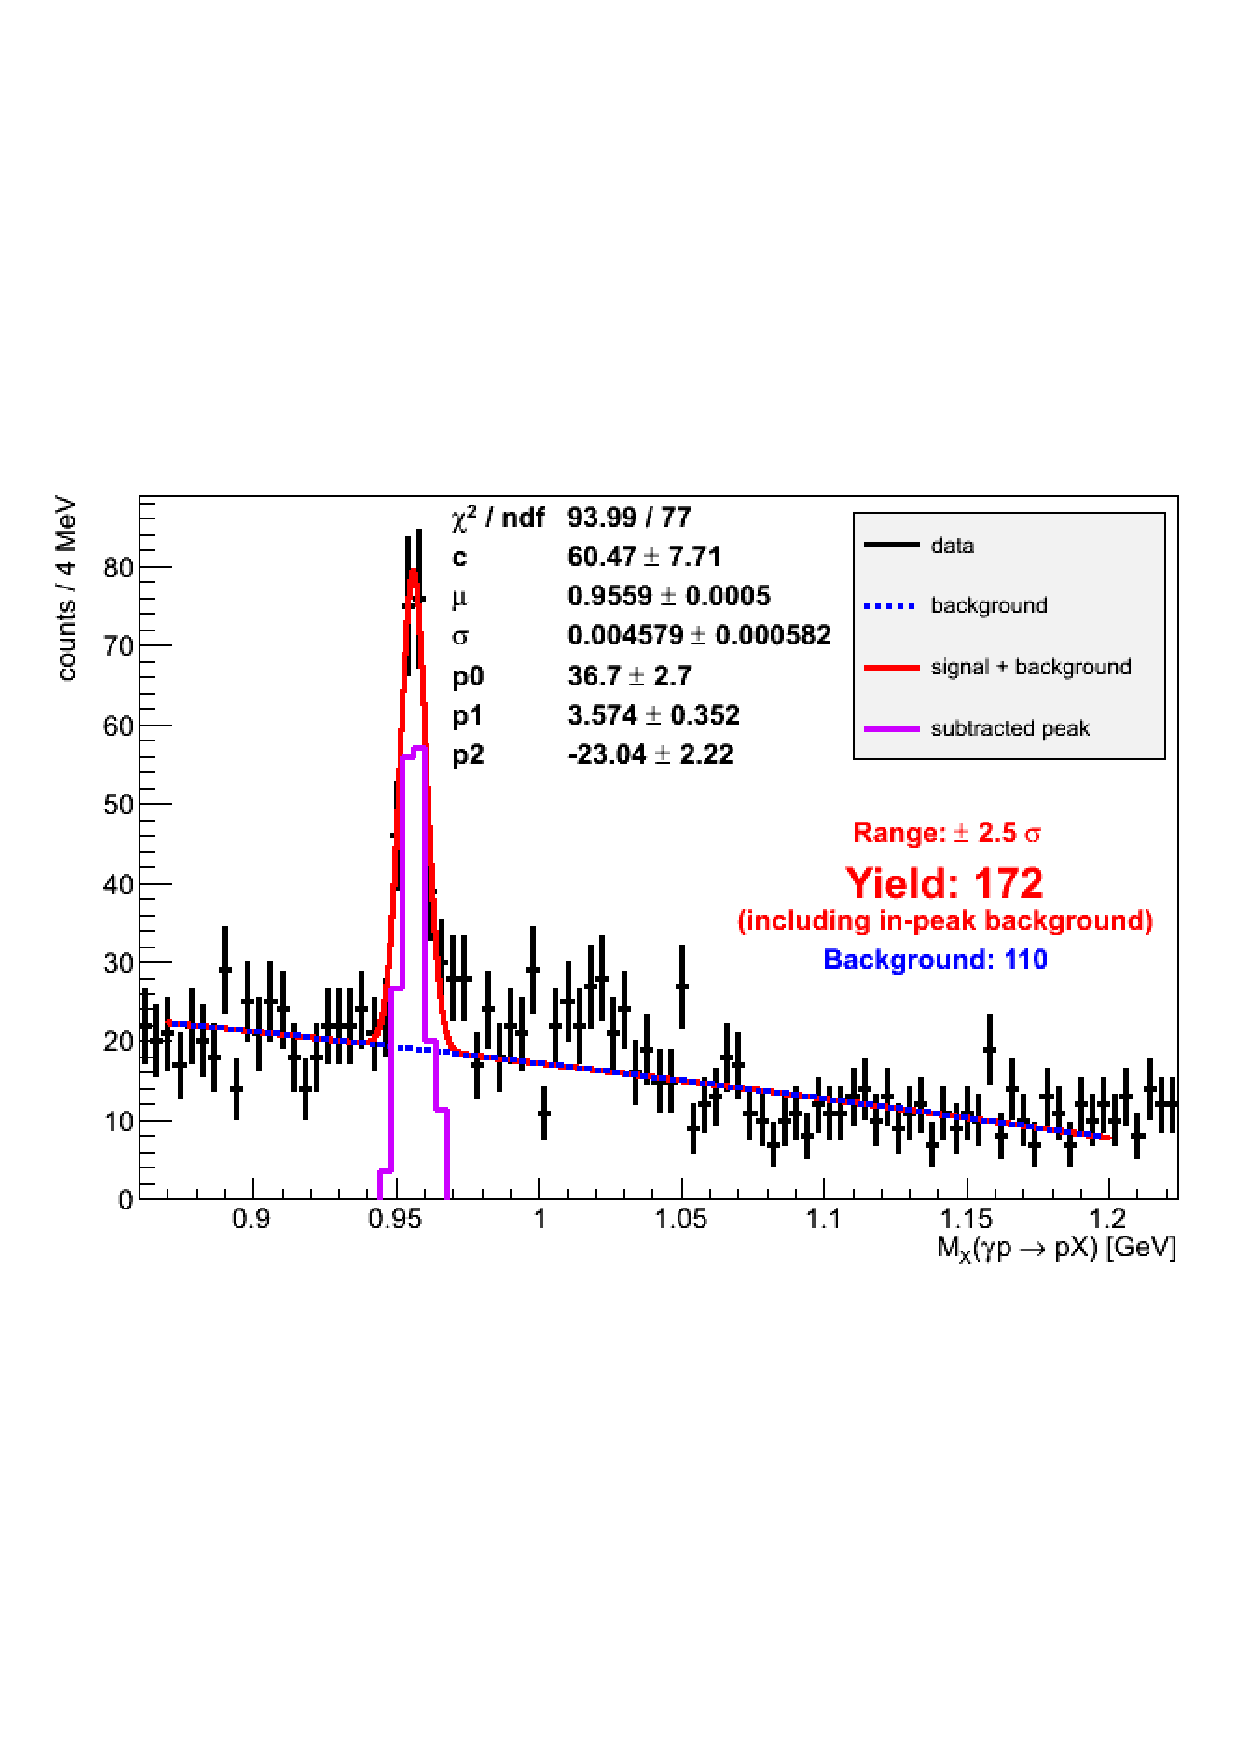
\includegraphics[width=160 pt]{figures/etaPeeg_mimass.pdf}}
\caption{(black)\textsc{\texttt{CLAS}} yield for $\gamma p \to p \eta^{\prime}  \to p e^+ e^- \gamma $ from g12 data set. (red line) Fit of signal and background using a Voigt signal and 1st order polynomial background function. (magenta line) Background subtracted signal peak, (blue dashed line) represents the background.}
\label{fig:etaP_ff}
\end{figure}
  A preliminary branching ratio $\Gamma(\eta^{\prime} \to  e^+ e^-  \gamma)$/$\Gamma(\eta^{\prime} \to  \gamma  \gamma)$ was measured to be consistent with the BESIII measurement. However, the statistics of either BESIII or CLAS are not ample enough to determine, statistically, which theoretical model best represents the structure of the $\eta^{\prime}$ meson~\cite{bib10,bib11,bib12}. Table~\ref{tab:etaP.models} outlines the current measurements and theoretical predictions.
\begin{table}[h!]
\begin{minipage}{\textwidth}
\begin{center}


\caption{\label{tab:etaP.models}LMD planned measurements \vspace{0.75mm}}
\begin{tabular}{cc}
%\begin{tabular}{p{5cm} | p{7cm}}
\hline
Charge radius $\left< r\right>$ & Masurement (M) / Prediction (P) \\
\hline
CLAS ($\eta^{\prime}\to e^+e^-\gamma$)   & TBD \\
BESIII ($\eta^{\prime}\to e^+e^-\gamma$)   & (M) $1.60\pm0.17(stat)\pm0.08(sys) \mathrm{GeV}^{-2}$~\cite{bib7} \\
CELLO ($\eta^{\prime}\to \mu^+\mu^-\gamma$)   & (M)  $1.7\pm0.4 \mathrm{GeV}^{-2}$~\cite{bib9}  \\
Dispersion    & (P)  $1.53^{0.15}_{-0.08} \mathrm{GeV}^{-2}$~\cite{bib12}  \\
ChPT    & (P) $1.6 \mathrm{GeV}^{-2}$~\cite{bib11}  \\
VMD    & (P) $1.45  \mathrm{GeV}^{-2}$~\cite{bib10}  \\
\hline 
\end{tabular}


\end{center}
\end{minipage}
\end{table}
\vspace{20pt}
\FloatBarrier
\subsection{Future Measurement of the $\eta^\prime$ Meson Transition Form Factor with \textsc{\texttt{CLAS12}}}
With the newly built \textsc{\texttt{CLAS12}} detector, $e^{\pm}$ identification can be achieved with a $e^{+}e^{-}/\pi^{+}\pi^{-}$ rejection of  $10^{6}-10^{11}$ while retaining $e^+ e^- \gamma$ acceptance $\sim 1 \% - 0.1 \%$.
%, Figure~\ref{fig:clas12} depicts the \textsc{\texttt{CLAS12}} detector and its subsystems.
%\begin{figure}[h!]
%\centerline{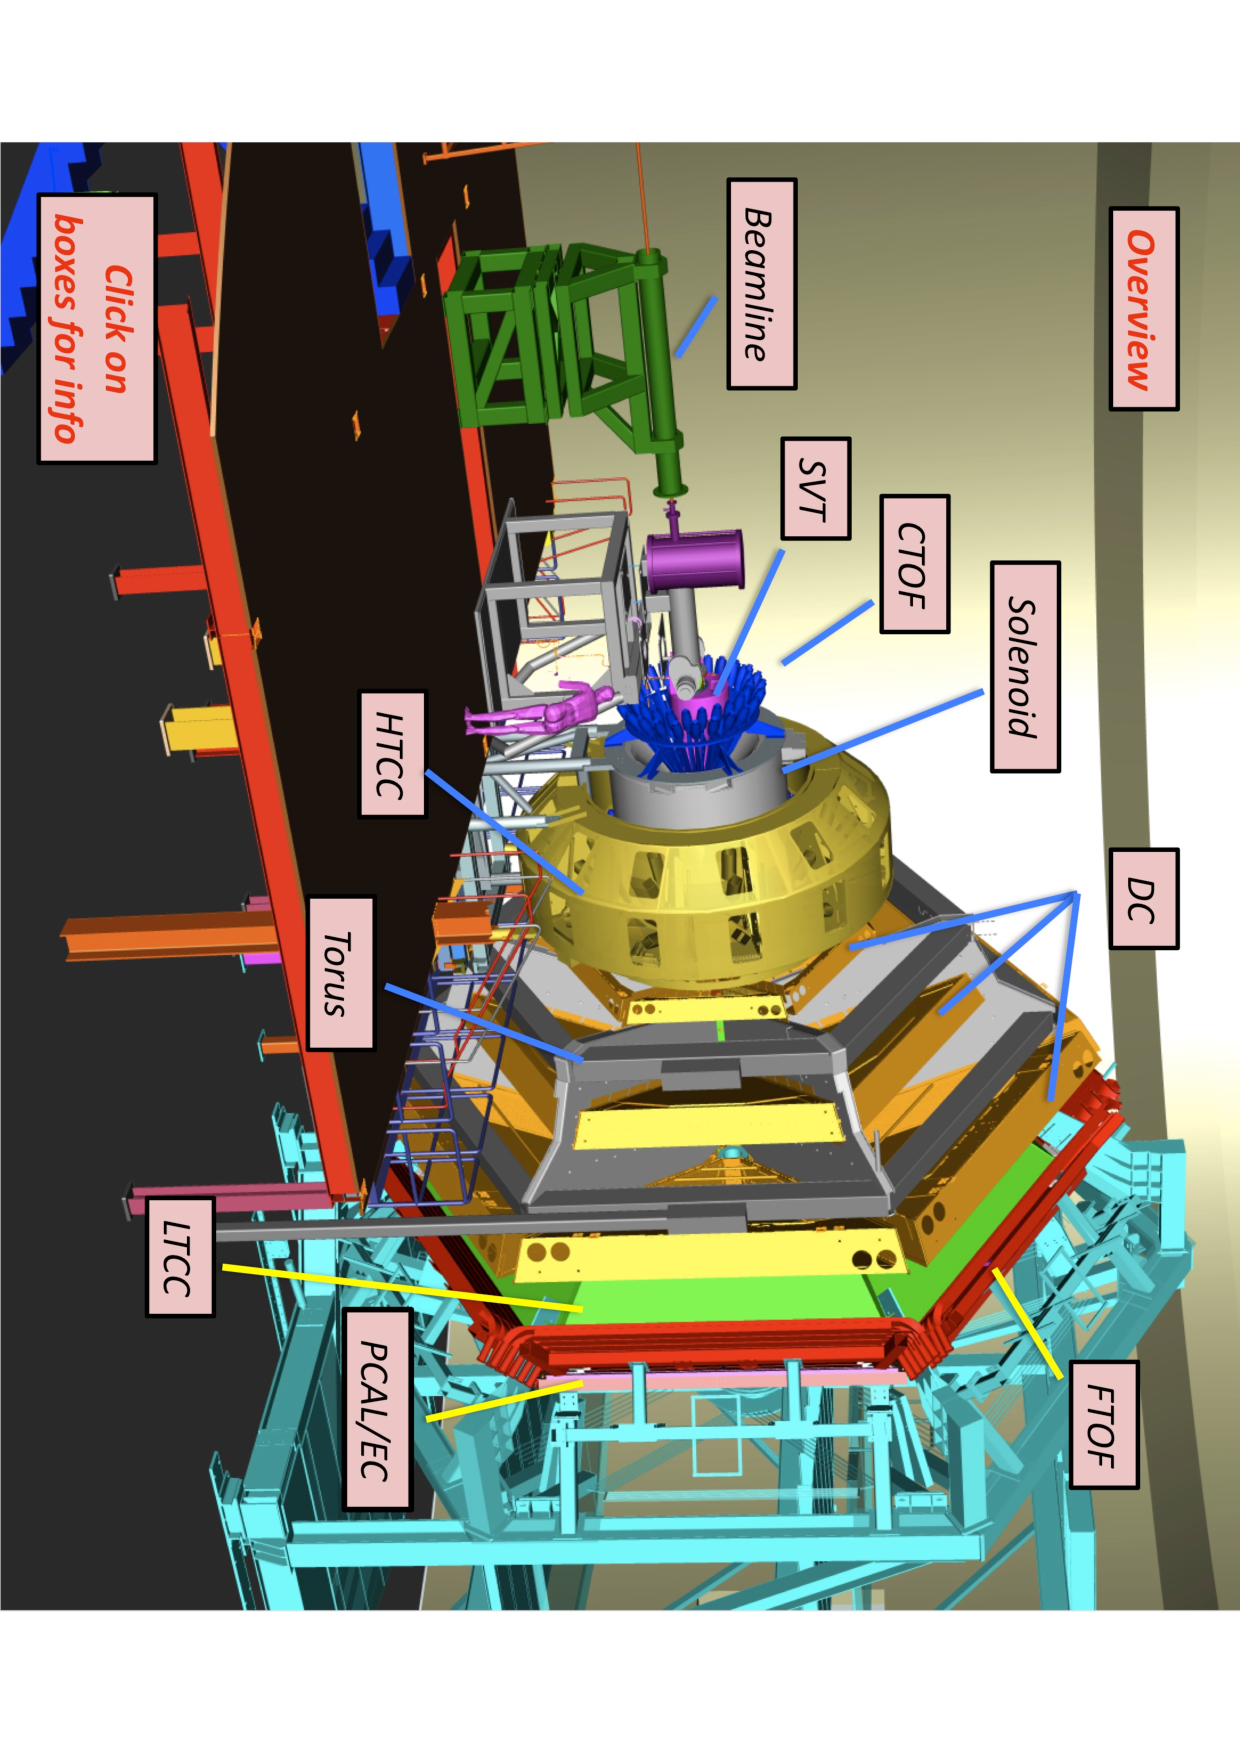
\includegraphics[angle = 90,width=225 pt]{figures/clas12-design.pdf}}
%\caption{The CEBAF Large Acceptance Spectrometer (\textsc{\texttt{CLAS12}})\\~(https://www.jlab.org/Hall-B/clas12-web/)}
%\label{fig:clas12}
%\end{figure}
\FloatBarrier
Using the \textsc{\texttt{CLAS12}} FASTMC simulation, a simulation of $10^6$ $e p \to e^{\prime} p \eta^{\prime}  \to p e^+ e^- \gamma (e^{\prime})$ was performed. The generation of events included cross-section information obtained from previous \textsc{\texttt{CLAS}} measurements, the $s^n$ scaling law on the cross-section and the VMD model for the decay of the $\eta^{\prime}$ meson to achieve a reasonable model of the production of the $\eta^{\prime} $ meson. Estimations of the integrated quasi-real photon rate from an electron beam of luminosity $10^{35}cm^{-2}s^{}-1$ impinged on a 5~cm $\ell H_2$ target yielded that the production rate for hadrons to be 80~kHz. Therefore, the total rate of $\eta^{\prime}$ can be calculated by defining the following ratio $R(W)$: 
\begin{equation}
R(W) = \frac{\sigma(W)}{\eta^{\prime} \text{ integrated } \sigma(W)}
\label{XsecR}
\end{equation}
and scaling the total rate by $R(W)$. This leads to:
\begin{equation}
\eta^{\prime}\text{ total rates / 80 Days }(W) = 80\,\rm{kHz}\cdot \frac{6.912e\cdot10^6\mathrm{\ seconds}}{\text{80 days}}\cdot \frac{1}{R(W)}
\label{etaPRate}
\end{equation}
The total $\etaP\rightarrow\epem\gamma$ rates per 80 days, and as a function $W$, is calculated by multiplying Eq.\ref{etaPRate} with the product of the average detection efficiency $\epsilon\approx 5\%$ as well as the branching fraction $\mathcal{BR} = 4.69\cdot10^{-4}$~\cite{bib7} for $\etaP\rightarrow\epem\gamma$. The total number $N_{tot}$ of expected $\etaP\rightarrow\epem\gamma$ events after 80 days of measurement is given by the integral of Eq.~\ref{etaPRate} over $W$. This leads to the expected yield:

\begin{equation}
  N_{tot} = \int\limits_{1.9\,\rm{GeV}}^{2.8\,\rm{GeV}} \Big[ {\color{red}{N(W)_{\etaP\rightarrow\epem\gamma\text{ / 80 Days }}}} \Big]dW = \mathrm{\frac{28,200 \ events}{80 Days}}
\label{yield}
\end{equation}
%This will give greater insight into the structure of the $ \eta^{\prime} $ meson than previously measured. 

\begin{figure}[h!]\begin{center}
		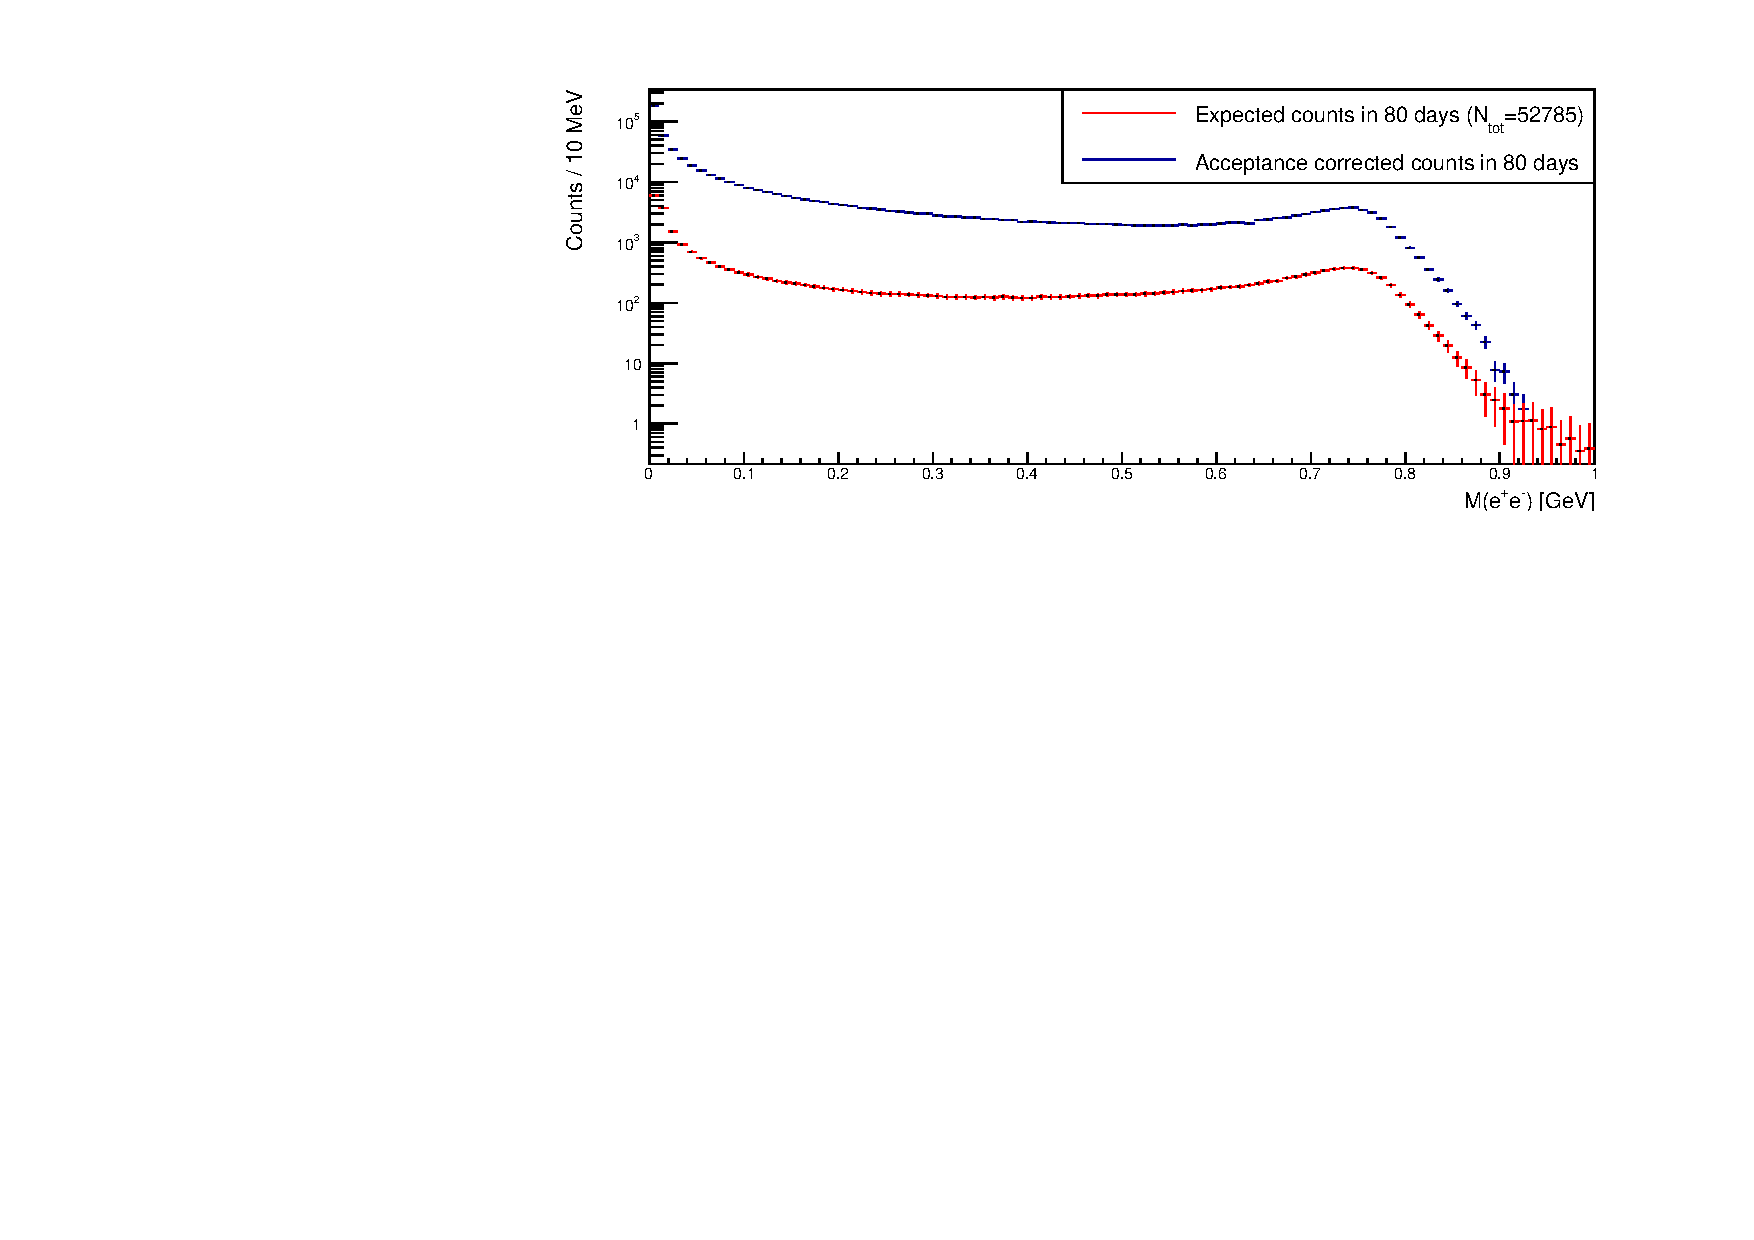
\includegraphics[width=250 pt, height=155 pt]{figures/counts.pdf}
		\caption[Acceptance as a function of $M(\epem)$]{\label{fig:counts}{(Color Online)Expected yield as a function of $M(\epem)$.}}
	\end{center}\end{figure}

	\begin{figure}[h!]\begin{center}
			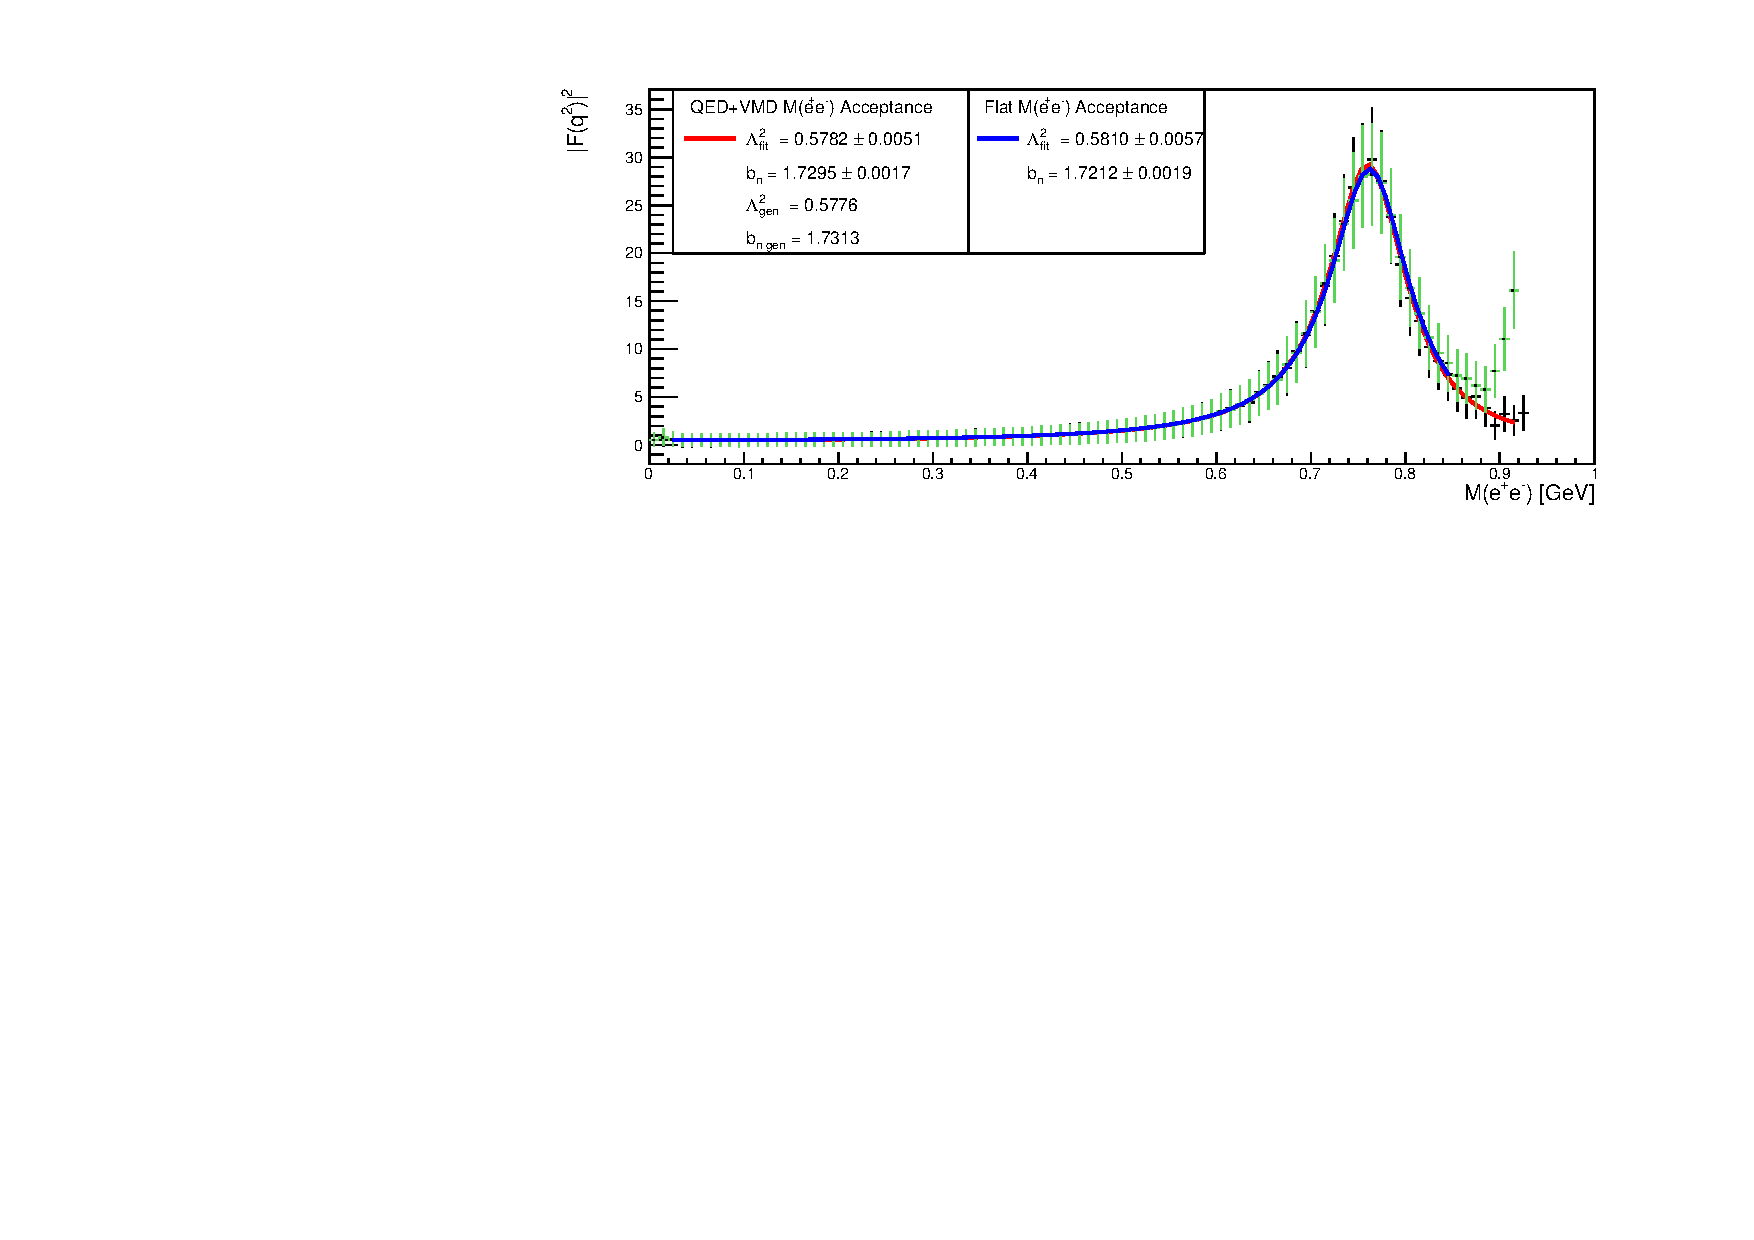
\includegraphics[width=225 pt, height=155 pt]{figures/result.pdf}
			\caption[TFF as a function of $M(\epem)$]{\label{fig:results}{(Color Online)$\left|F(q^2)\right|^2$ as a function of $M(\epem)$ using two acceptance models. (black points) QED+VMD $M(\epem)$ acceptance model. (green points) Flat $M(\epem)$ acceptance model. The solid lines represent a fit using Eq.~\ref{eq:cpole} to the data points.}}
		\end{center}\end{figure}

	\FloatBarrier
From Fig.~\ref{fig:counts} the QED normalized spectrum can be deduced and is shown in Fig.~\ref{fig:results}. Both generation models (i.e. flat and QED+VMD) are used to determine the transition form factor. It is shown that there exists a systematic uncertainty depending on the chosen generation model. However, the final calculation on the slope parameter or the TFF shows a negligible impact of this uncertainty. Regardless of the generation model, it is shown in Fig.~\ref{fig:results} that the accumulated statistics collected by CLAS12 allow for a precision of each parameter $\lesssim 0.5\%$. Compared to current experimental uncertainties of 10\% and differences in theoretical approaches of $\approx$ 10\%, Table~\ref{tab:etaP.models}, therefore a measurement by CLAS12 would not only be in the position to decisively discriminate between the theoretical predictions, but also help to further constrain the hadronic light-by-light amplitude
to the muon g-2 anomaly~\cite{gminus2}.

% BibTeX or Biber users please use (the style is already called in the class, ensure that the "woc.bst" style is in your local directory)
% \bibliography{name or your bibliography database}
%
% Non-BibTeX users please use
%
\begin{thebibliography}{00}
%
% and use \bibitem to create references.
%
%\bibitem{RefJ}
%% Format for Journal Reference
%F.~Author~\textit{et al.}, Journal \textbf{Volume}, page numbers (year) {\em{no trailing dot!}}
%% Format for books
%\bibitem{RefB}
%Book Author, \textit{Book title} (Publisher, place, year) page numbers {\em{no trailing dot!}}
%\bibitem{bib0}
%P. Adlarson \textit{et al.}, Physics Letters B, 707, 243 - 249, 2012	
%% etc

\bibitem{bib2}
A.~Abele et~al.
\newblock {\em Physics Letters B}, 402:195 -- 206, 1997.

\bibitem{bib7}
M.~Ablikim et~al.
\newblock {Observation of the Dalitz Decay $\eta' \to \gamma e^+e^-$}.
\newblock {\em Phys. Rev.}, D92(1):012001, 2015.

\bibitem{bib0}
P.~Adlarson et~al.
\newblock {\em Physics Letters B}, 707:243 -- 249, 2012.

\bibitem{lmdCAA}
M.~Amaryan et~al.
\newblock {\em Photoproduction and \uppercase{D}ecay of \uppercase{L}ight
  \uppercase{M}esons in \uppercase{CLAS}}.

\bibitem{bib11}
Ll. Ametller et~al.
\newblock Transition form factors in ${\ensuremath{\pi}}^{0}$,
  $\ensuremath{\eta}$, and ${\ensuremath{\eta}}^{\ensuremath{'}}$ couplings to
  $\ensuremath{\gamma}{\ensuremath{\gamma}}^{*}$.
\newblock {\em Phys. Rev. D}, 45:986--989, 1992.

\bibitem{bib5}
R.~Arnaldi et~al.
\newblock Study of the electromagnetic transition form-factors in and decays
  with \{NA60\}.
\newblock {\em Physics Letters B}, 677(5):260 -- 266, 2009.

\bibitem{bib1}
D.~Babusci et~al.
\newblock {\em Physics Letters B}, 718:910 -- 914, 2013.

\bibitem{gminus2}
Thomas Blum et~al.
\newblock {The Muon (g-2) Theory Value: Present and Future}.
\newblock 2013.

\bibitem{bib10}
A.~Bramon and E.~Massó.
\newblock Q2-duality for electromagnetic form factors of mesons.
\newblock {\em Physics Letters B}, 104(4):311 -- 314, 1981.

\bibitem{bib12}
C.~Hanhart et~al.
\newblock {Dispersive analysis for $\eta\to \gamma\gamma^*$}.
\newblock {\em Eur. Phys. J.}, C73(12):2668, 2013.

\bibitem{bib4}
Norman~M. Kroll and Walter Wada.
\newblock Internal pair production associated with the emission of high-energy
  gamma rays.
\newblock {\em Phys. Rev.}, 98:1355--1359, 1955.

\bibitem{Kubis2015}
Bastian Kubis and Judith Plenter.
\newblock Anomalous decay and scattering processes of the $\eta$ meson.
\newblock {\em The European Physical Journal C}, 75(6):1--12, 2015.

\bibitem{Schneider}
Sebastian~P. Schneider et~al.
\newblock {The $\omega -> \pi^0 \gamma^*$ and $\phi -> \pi^0 \gamma^*$
  transition form factors in dispersion theory}.
\newblock {\em Phys. Rev.}, D86:054013, 2012.

\bibitem{bib6}
Carla Terschlusen and Stefan Leupold.
\newblock Electromagnetic transition form factors of light vector mesons.
\newblock {\em Physics Letters B}, 691(4):191 -- 201, 2010.

\bibitem{bib8}
M.~Williams et~al.
\newblock {Multivariate side-band subtraction using probabilistic event
  weights}.
\newblock {\em JINST}, 4:P10003, 2009.

\end{thebibliography}

\end{document}

% end of file template.tex

